\section{General structure}
The internal structure are divided into four explicit phases and this chapter will provide an indepth explanation of each of the phases. But in short the following is done:
\begin{itemize}
\item In the JModelica phase the provided model is compiled and linearised before extracting a Mathematical model used to create the SFG.
\item In the next phase, Intermediate representation, the obtained mathematical model is converted to an SFG representation used internally by the export tool. 
\item The internal representation of the SFG is then analysed, checking for inconsistencies or possible problems that might origin from the original Modelica model, before user provided transformations are applied. 
\item Finally  the  SFG representation, used internally, is translated to the actual XML based representation used in ProMoVis.
\end{itemize}
A brief overview is provided in Fig.~\ref{fig:phase}. The four phases have been kept strongly separated  from each other, to make room for adding user interaction in-between them. Although not currently utilized, the main reason for this is that, during the course of the project, a lot of questions have been raised regarding how to handle certain situations from a user perspective. Ranging from what to do when a compile time error occurs and what to do if the system is unstable at the linearisation, to  which states actually is of interest to analyse in ProMoVis and how the graphical representation should be created. Unfortunately, these kind of user experience questions, were not possible to address within the project. 
\begin{figure}[h]
\fbox{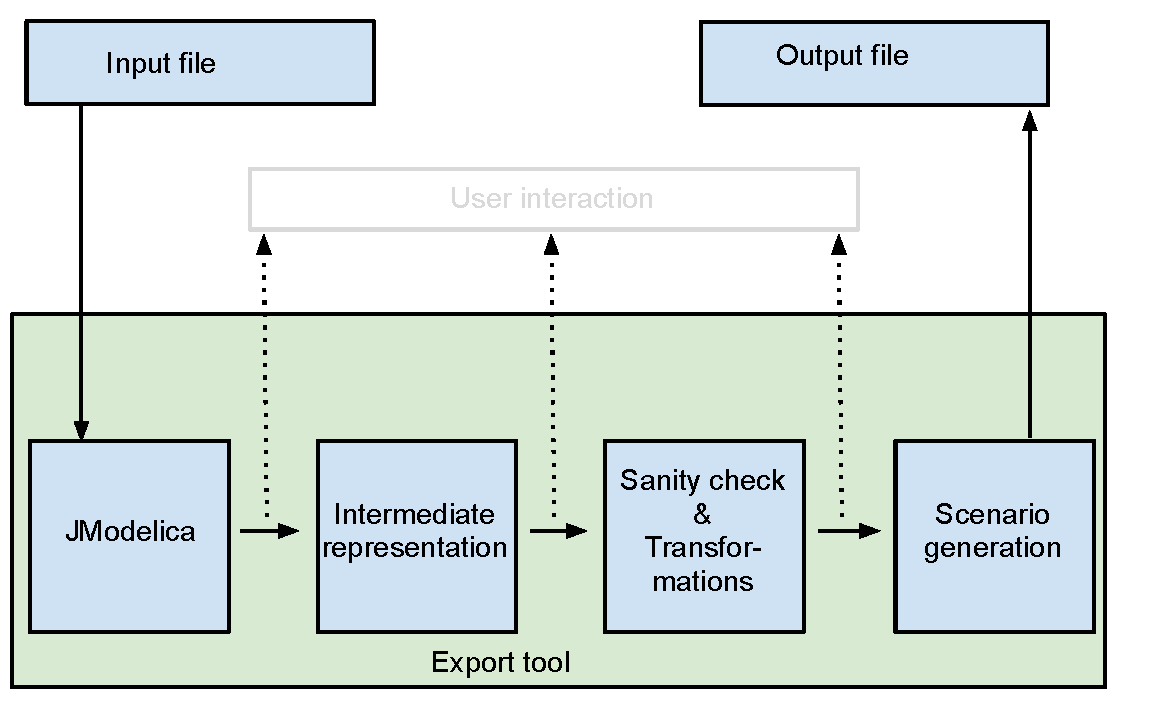
\includegraphics[scale=0.8,bb=0 0 7.72in 4.75in] {Figures/phases.pdf}}
\caption{Diagram of the internal structure of the export tool.}
\label{fig:phase}
\end{figure}

\subsection{Interfacing with the tool}
Since there are several separate phases in the tool, and each of the phases might later be extended with additional options and necessary parameters, XML is used to pass information to the tool. By using XML that is a well known, structured, format for representing data there is not only the benefit of making the inputfiles easy accessible to other developers and software, but also it elmininates the need to develop and maintain the code for parsing a tool specific format. With XML, existing software for parsing and object representation of the XML files can be used. And in the tool, an instance, of the whole or parts of the inputfile can be passed along to each of the phases. Where each phase then may just extract the necessary parameters. \\\newline %
In the example file,  Fig.~\ref{fig:coding},  %
the \textit{filepath} and \textit{model} nodes are the path to the original Modelica source file and the full model name, including packagename. The node \textit{mpattern} is used to provide information regarding which of the variables declared in the Modelica model that should be measured variables in the output file. This is achieved through providing one or more regular expressions that the tool will try to match to the ending of the variable names. E.g. if the tool encounters the variables foo\_pmv, foo\_foobar, foox2 or x2 it will indicate that those variables should become measured variables in the final ProMoVis representation.
%
\begin{figure}
\lstset{language=XML}
\begin{lstlisting}
<?xml version="1.0" ?> 
<root>
        <filepath>C:\Users\Public\Documents\QuadTankPack.mo</filepath>
        <model>QuadTankPack.QuadTank</model>
        <mpattern>_pmv;_fooBar;x2</mpattern>
        <outputpath>C:\ProMoVis\output.xml</outputpath>
        <pmvoutputpath>C:\ProMoVis\QuadTank.pmv</pmvoutputpath>
</root>
\end{lstlisting}
\caption{Example inputfile used to pass information to the tool.}
\label{fig:coding}
\end{figure} 
%

\subsection{JModelica(Compile)Phase}
The JModelica environment is used to compile the Modelica models to JModelicas JMU representation \cite{jmodelicaorg}\nocite{*}. ProMoVis assumes the systems to be linear and the compiled model needs to be linearised around an operating point. The linearisation is performed at time 0, and it is assumed that the system is stable at that time.\\\\After linearisation a DAE on the following form can be extracted:%
\begin{equation}
E\dot{x} = Ax + Bu + Fw + g
\end{equation}%
This represenation should be familiar, the $x$ and $\dot{x}$  vectors represents the states and outputs of the linearized system. The $u$ vector represents declared inputs and the $w$ vector represents algebraic variables, that is all variables in the original model that has no derivative declared. Finally $g$ is a constant bias vector.\\\\The linearisation also outputs some useful information that we later use in the generation of the ProMoVis scenarios:
\begin{itemize}
\item \textit{State names}, corresponding to the declared variable names from the original Modelica file.
\item \textit{Input names}, corresponding to the declared input names from the original Modelica file.
\item \textit{Algebraic names}, corresponding to the declared algebraic variable names from the original Modelica file.
\item \textit{Operating points} for the linear model \textit{dx0},\textit{w0}, \textit{u0} and \textit{x0}. In later stages this information is used to provide feedback to the user regarding the validity of the resulting model.
\end{itemize}
From now on we will refer to states and algebraic variables as simply "variables" and whenever a distinction between the two is needed, it will be explicitly declared.% 
\subsection{Generation of the internal structure}
When the DAE is obtained, the task is then to extract the relations between the variables from it. The tool collects and stores each of the variables, together with each of the variables that acts as inputs to it. Although it might feel more natural to store a variable together with each of the variables that it affects, this representation was choosen since ProMoVis supports both of the representations but it is straightforward, from the DAE, to solve a variable for all its inputs.\\\newline
This fact is easilly seen with the following example.\\\newline
The DAE for a model with two state variables, two inputs and and two algebraic variables could be described by the following general structure:
%
\begin{equation}\begin{bmatrix} E_{11} & E_{12} \\ E_{21} & E_{22} \\ E_{31} & E_{32} \\ E_{41} & E_{42} \end{bmatrix} \left[ \begin{array}{c} \dot{x_0} \\ \dot{x_1} \end{array} \right] = \begin{bmatrix} A_{11} & A_{12} \\ A_{21} & A_{22} \\ A_{31} & A_{32} \\ A_{41} & A_{42} \end{bmatrix} \left[ \begin{array}{c} x_0 \\ x_1 \end{array} \right] + \begin{bmatrix} B_{11} & B_{12} \\ B_{21} & B_{22} \\ B_{31} & B_{32} \\ B_{41} & B_{42} \end{bmatrix} \left[ \begin{array}{c} u_0 \\ u_1 \end{array} \right]+\begin{bmatrix} F_{11} & F_{12} \\ F_{21} & F_{22} \\ F_{31} & F_{32} \\ F_{41} & F_{42}\end{bmatrix} \left[ \begin{array}{c} w_0 \\ w_1 \end{array} \right]\end{equation}
%
The task is now, to find which of the rows in the system that should be solved for which variable so that the whole system can be solved. Here a demand is that the DAE may not contain any Algebraic loops. For a more thorough discussion regarding this and the decision of which row to solve for which variable please review Appendix \ref{appA}.\\\newline After deciding which row that should be solved for which of the variables we build up an intermediate representation of the SFG, used internally in the tool, where we store each of the variables together with all of its input variables. This is best explained with the help of an example, if we assume that we should solve row 1 for x0 the procedure is, after laplace transformation, as follows:
%
\begin{equation}
\begin{array}{rcl} E_{11}x_0s  +E_{12}x_1s=A_{11}x_0  +A_{12}x_1 +B_{11}u_0  +B_{12}u_1  +F_{11}w_0  +F_{12}w_1 
\end{array}
\end{equation}\\
%
Putting $x_0$ alone on the left-hand side and collecting the coefficients then yields:%
\begin{equation}
\begin{array}{rcl} (E_{11}s-A_{11})x_0  =(A_{12}-E_{12}s)x_1 +B_{11}u_0  +B_{12}u_1 +F_{11}w_0  +F_{12}w_1 
\end{array}
\end{equation}
%
Finally, solving for $x_0$ yields:
\begin{equation}
\begin{array}{rcl} x_0  = \frac{(A_{12}-E_{12}s)}{(E_{11}s-A_{11})}x_1 +\frac{B_{11}}{(E_{11}s-A_{11})}u_0  +\frac{B_{12}}{(E_{11}s-A_{11})}u_1 +\frac{F_{11}}{(E_{11}s-A_{11})}w_0 +\frac{F_{12}}{(E_{11}s-A_{11})}w_1
\end{array}
\end{equation}
%
Naturally, only the variables with non-zero coefficients are stored as input variables. For a complete overview of how the information retrieved from the Modelica is represented, please refer to the source code \cite{githabb}\nocite{*}. But for the continued discussion, the internal representation of a variable, equivalent to a node in the SFG can be viewed upon as depicted in Fig. ~\ref{fig:internalrep}. Where \textit{Variable} corresponds to a vertice in the SFG. It holds a dictionary, \textit{inputs}, with variable names as keys and the corresponding transfer functions as a values. These key-value pairs corresponds to the edges in the SFG going into the vertice. There is also additional, information that may be obtained from the Modelica models if provided, such as saturation values, operating points etc.%
%
\begin{figure}
\fbox{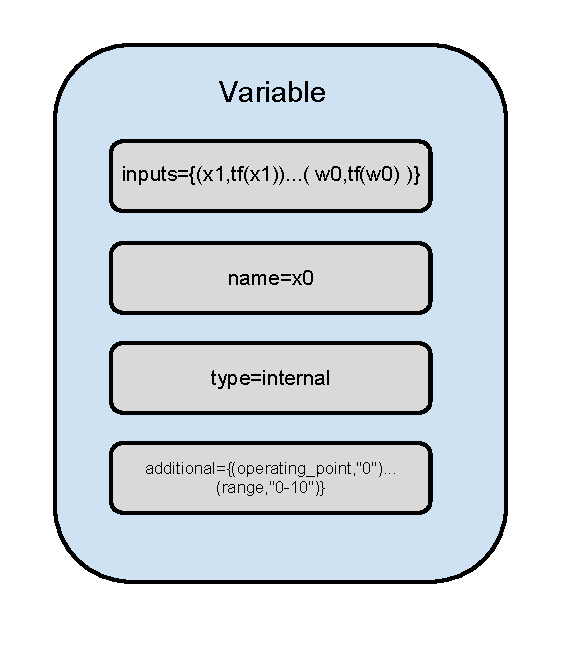
\includegraphics[scale=0.8,bb=0 0 97mm 111mm] {Figures/variable_structure.pdf}}\\\newline 
\caption{Overview of the information contained in the tools internal representation of a vertice}
\label{fig:internalrep}
\end{figure}
%
\subsection{Validation and Transformations}
After extracting the variables, we examine the value of the derivatives at the linearisation point. They should preferrably be 0, if they are different from 0 a warning is emitted so that the user is notified that the model they are using probably is not stable at the choosen linearisation point. It is also during this phase that additional modifications, provided by the user, should be done. Currently, the only modification supported, is the ability to indicate that some of the variables in the system should be emitted as measured variables in the resulting ProMoVis representation. By default, all variables declared as inputs, in the original Modelica model,  are emitted as controlled variables, while the other variables are emitted as internal variables.
\subsection{Scenario generation}
When the structure is validated and all optional transformations have been done. The actual generation of the ProMoVis represenation is straightforward. Basically the ProMoVis representation contains two parts. First the descriptive part, a collection of all variables, with their names, graphical layout and additional mathematical properties. The second part, the processmodels, are describing the relations between variables in the system. 
\subsubsection{Graphical Layout}
Even though Modelica supports description of position and graphical representation of models through its annotations interface, these are not necessary for a valid Modelica model. Therefore no effort has been put into trying to extract this type of meta-information. Instead, to make sure that a user of ProMoVis is able to easily access and attach controllers to the generated model the variables are emitted as depicted in Fig. ~\ref{fig:promosfg}. That is, control and measured variables are emitted as the upper and lower half of a circle respectively while internal variables, that are assumed not to be of interest to the user, are collected in the center of the circle. This is done due to the fact that no graphical semantics can be assumed to be available in the original modelica model and is achieved by a helper object, the layout emitter, that is initiated with the number of internal, measured and input variables and then calculates the step sizes in the x and y directions that will achieve the desired circular shape.
%
\begin{figure}
\fbox{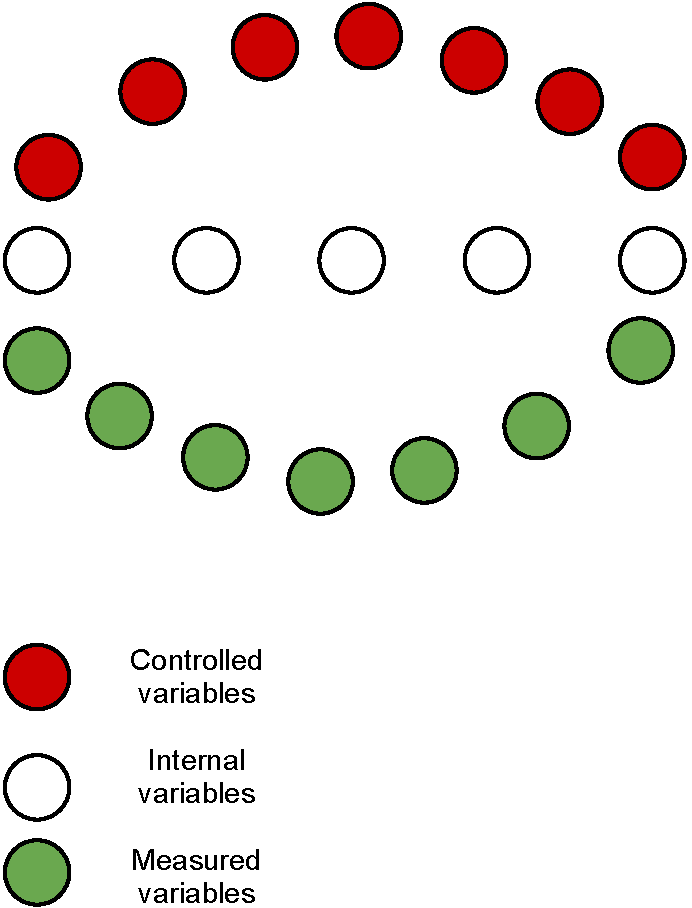
\includegraphics[scale=0.4,bb=0 0 117mm 154mm] {Figures/layout.pdf}}
\caption{Illustration of how the tools outputs the ProMoVis specific graphical representation of an SFG.}
\label{fig:promosfg}
\end{figure}
%  
\section{DAE vs ODE}
Readers familiar with Modelica and the JModelica environment might be accustomed to working with the ODE-representation of systems. The reason that the tool sticks with the DAE, even though the extraction of SFGs from an ODE is less complex, is due to the fact that when using the ODE we loose causality whenever a state depends on an algebraic variable. The DAE, although also lacking information, translates to an SFG that is more likely to resemble to structure of the original, physical, model that the user provided for export. For a more thorough discussion of this see Appendix \ref{appB}.


